\section{Grafici ed immagini}
\begin{figure}[h]
	\centering
	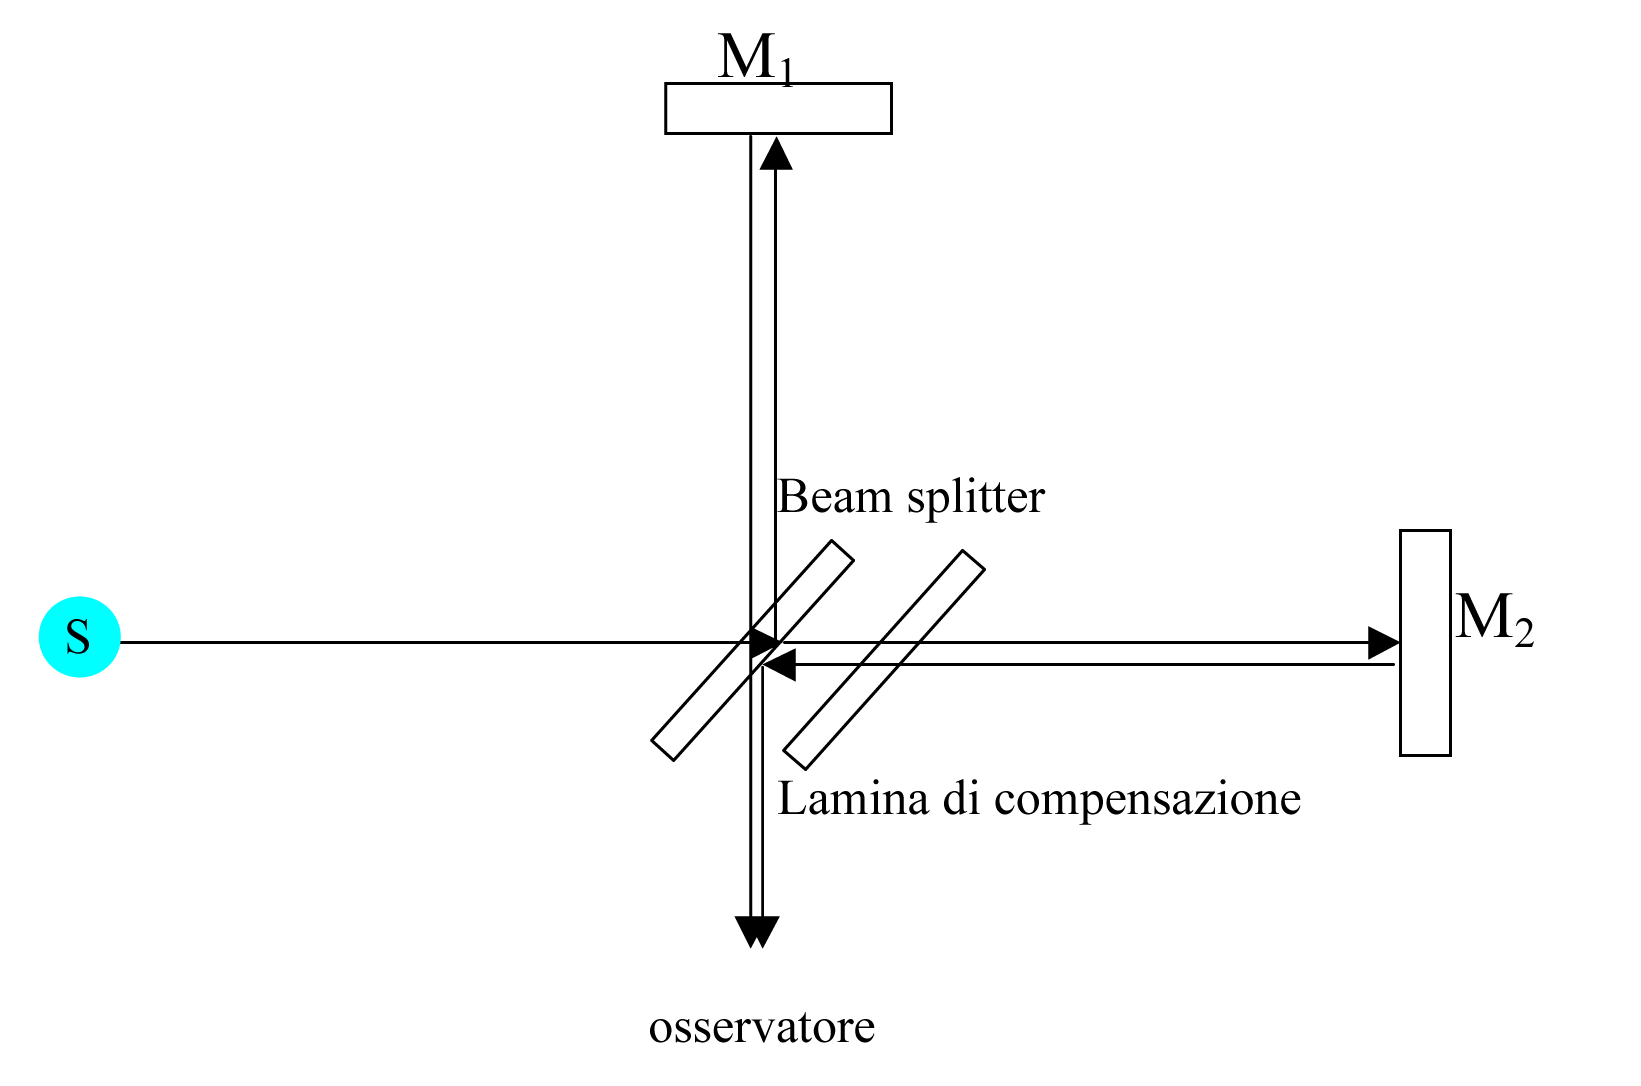
\includegraphics[scale=0.5]{Ottica 2B Interferometro di Michelson-1.png}
	\caption{Interferometro di Michelson}
	\label{f:figura_1}
\end{figure}
\begin{figure}[h]
	\centering
	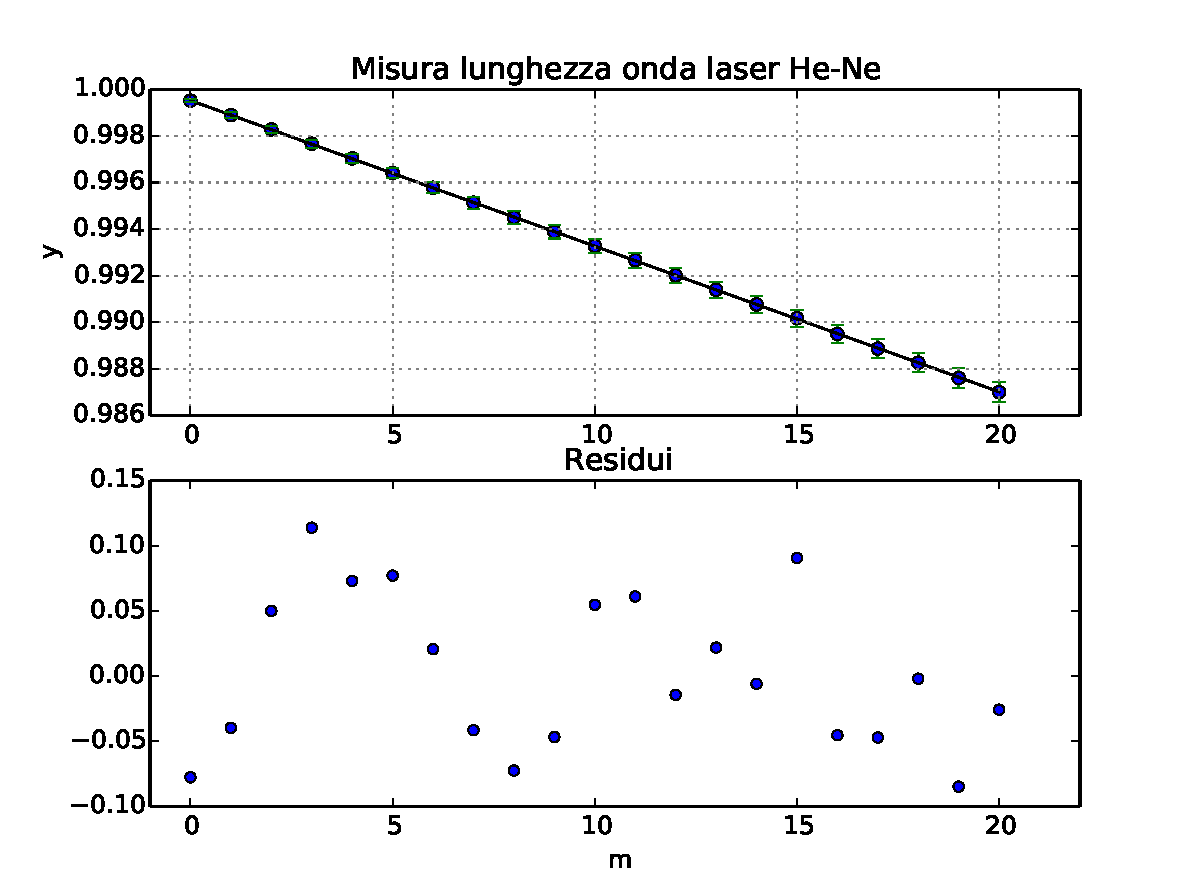
\includegraphics[scale=0.5]{grafico.pdf}
	\caption{Grafico del coseno in funzione dell'ordine di diffrazione.}
           \label{f:figura_2}
\end{figure}

\begin{figure}[h]
	\centering
	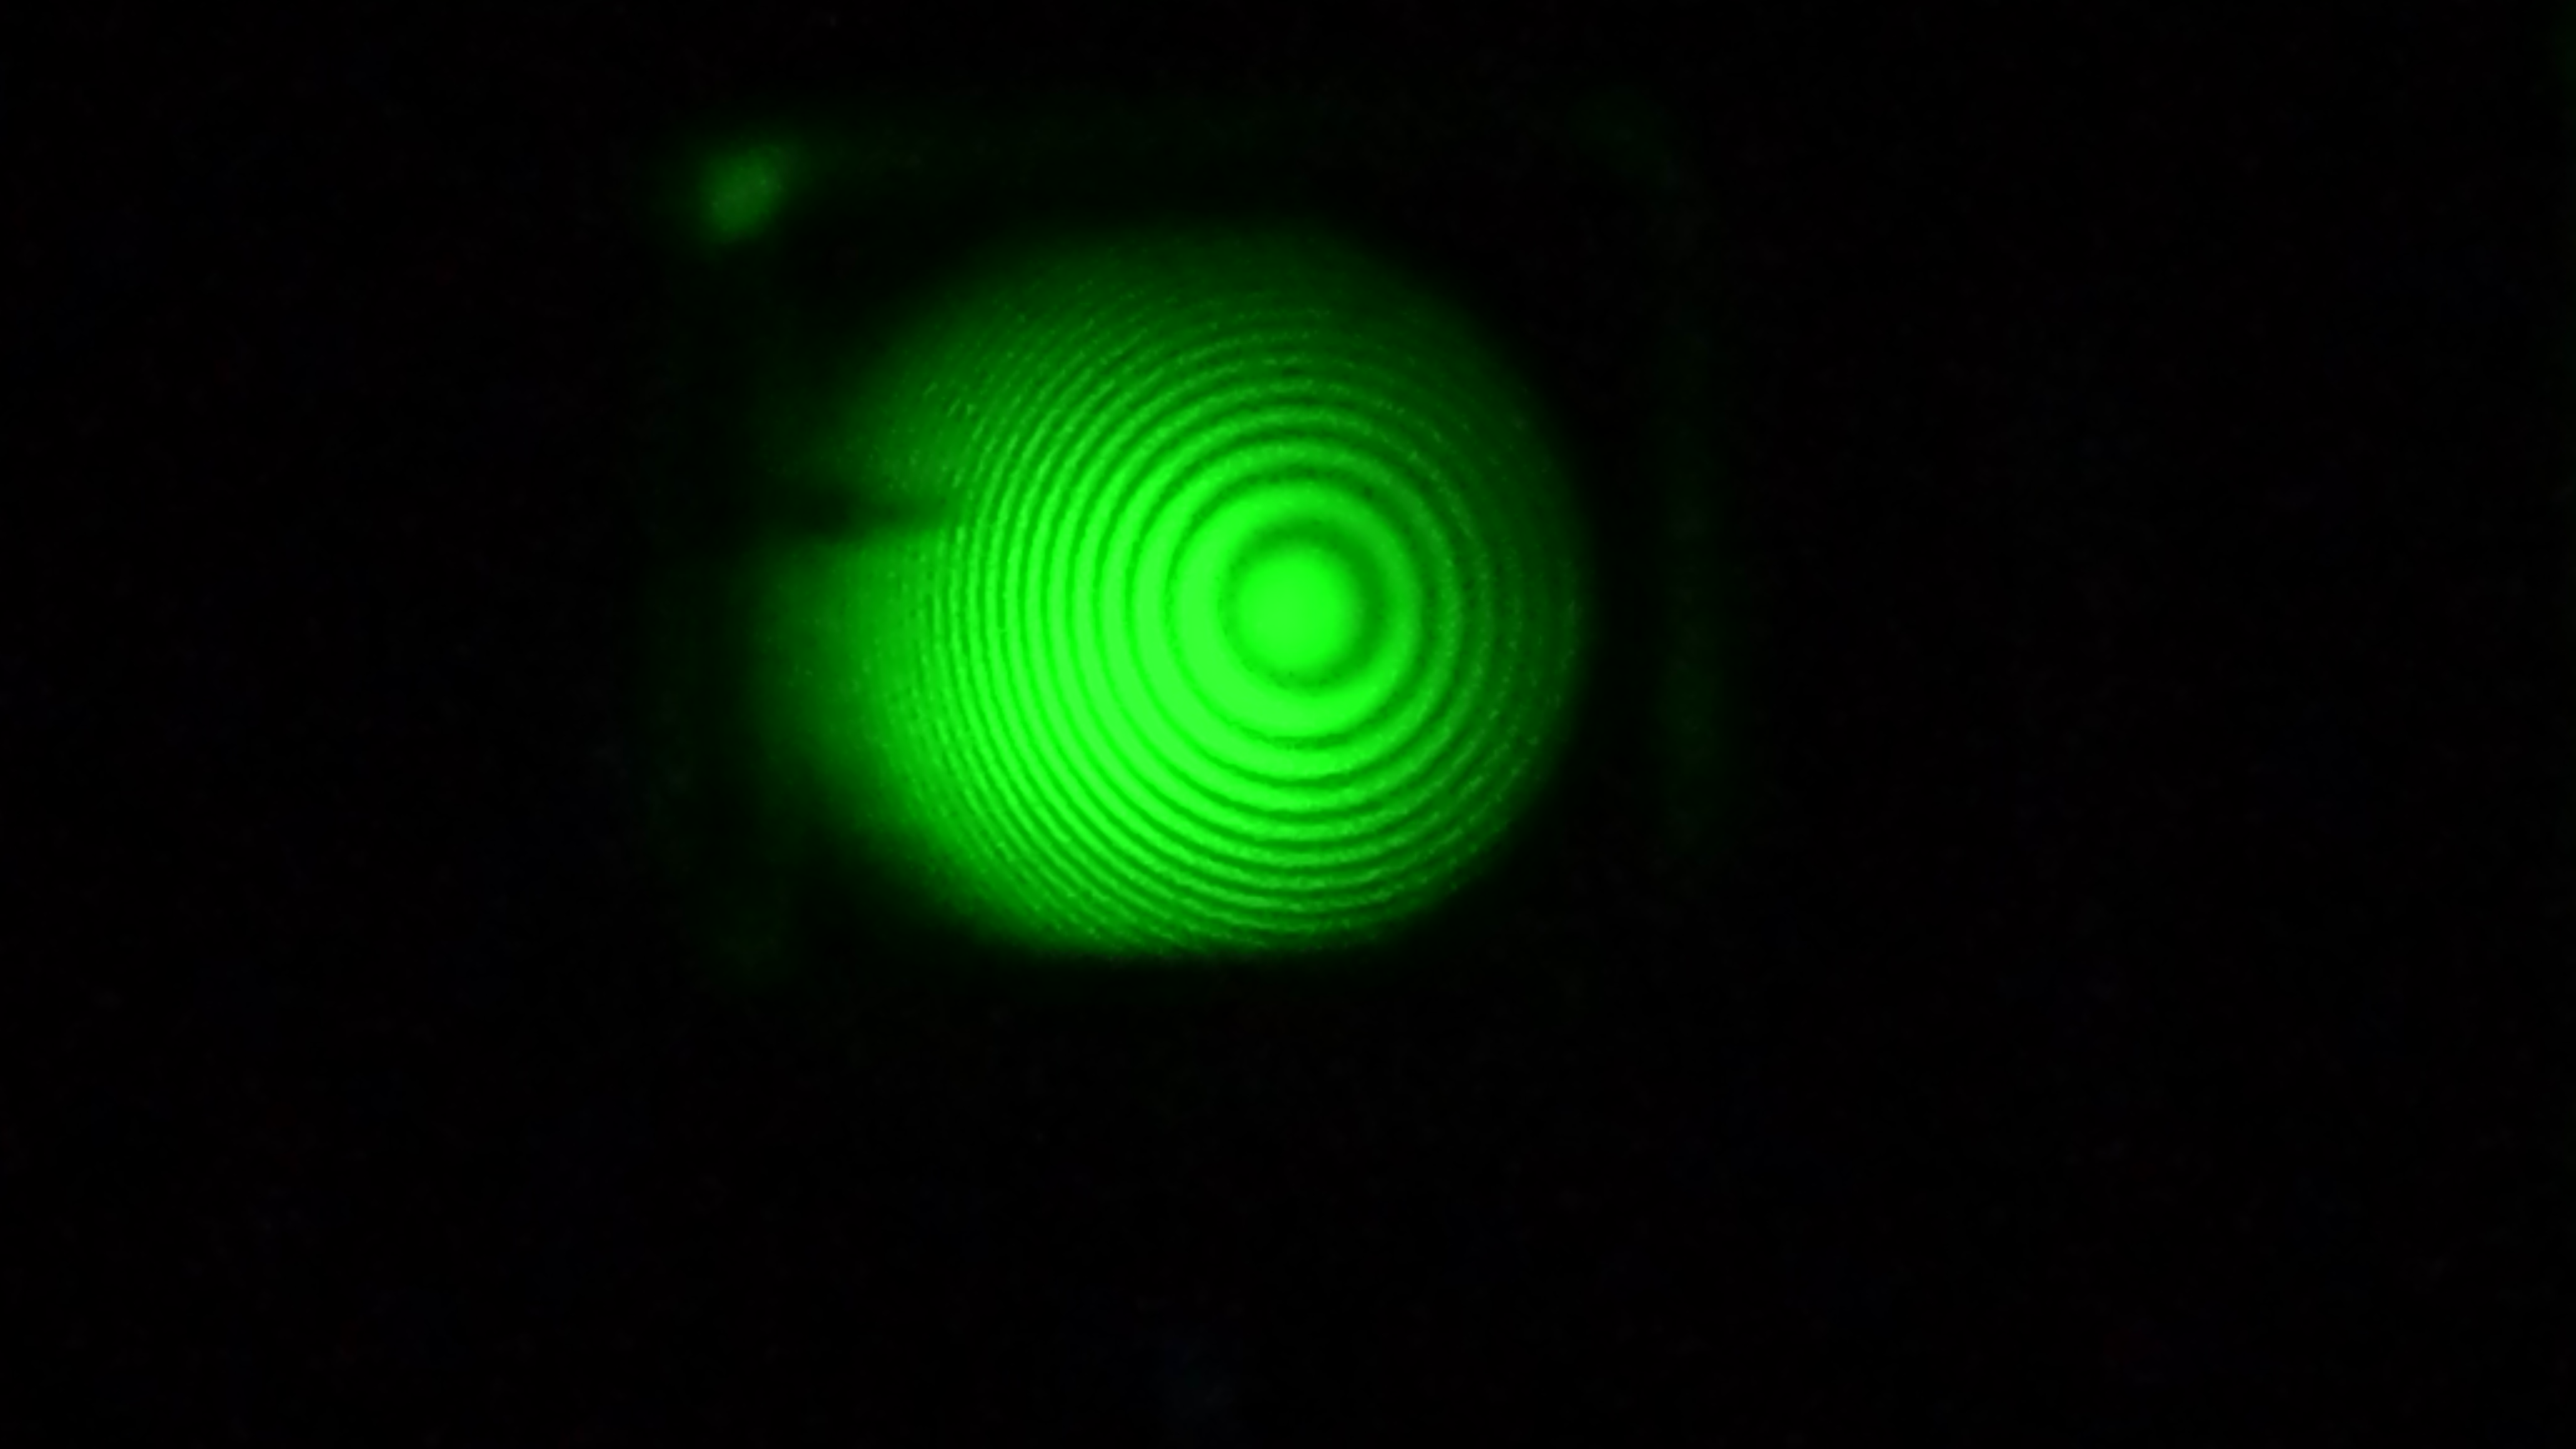
\includegraphics[scale=0.5]{frange_mercurio.pdf}
	\caption{Frange determinate dalla luce verde emessa dal mercurio osservate all'uscita dell'interferometro}
           \label{f:frange_mercurio}
\end{figure}

\begin{figure}[h]
	\centering
	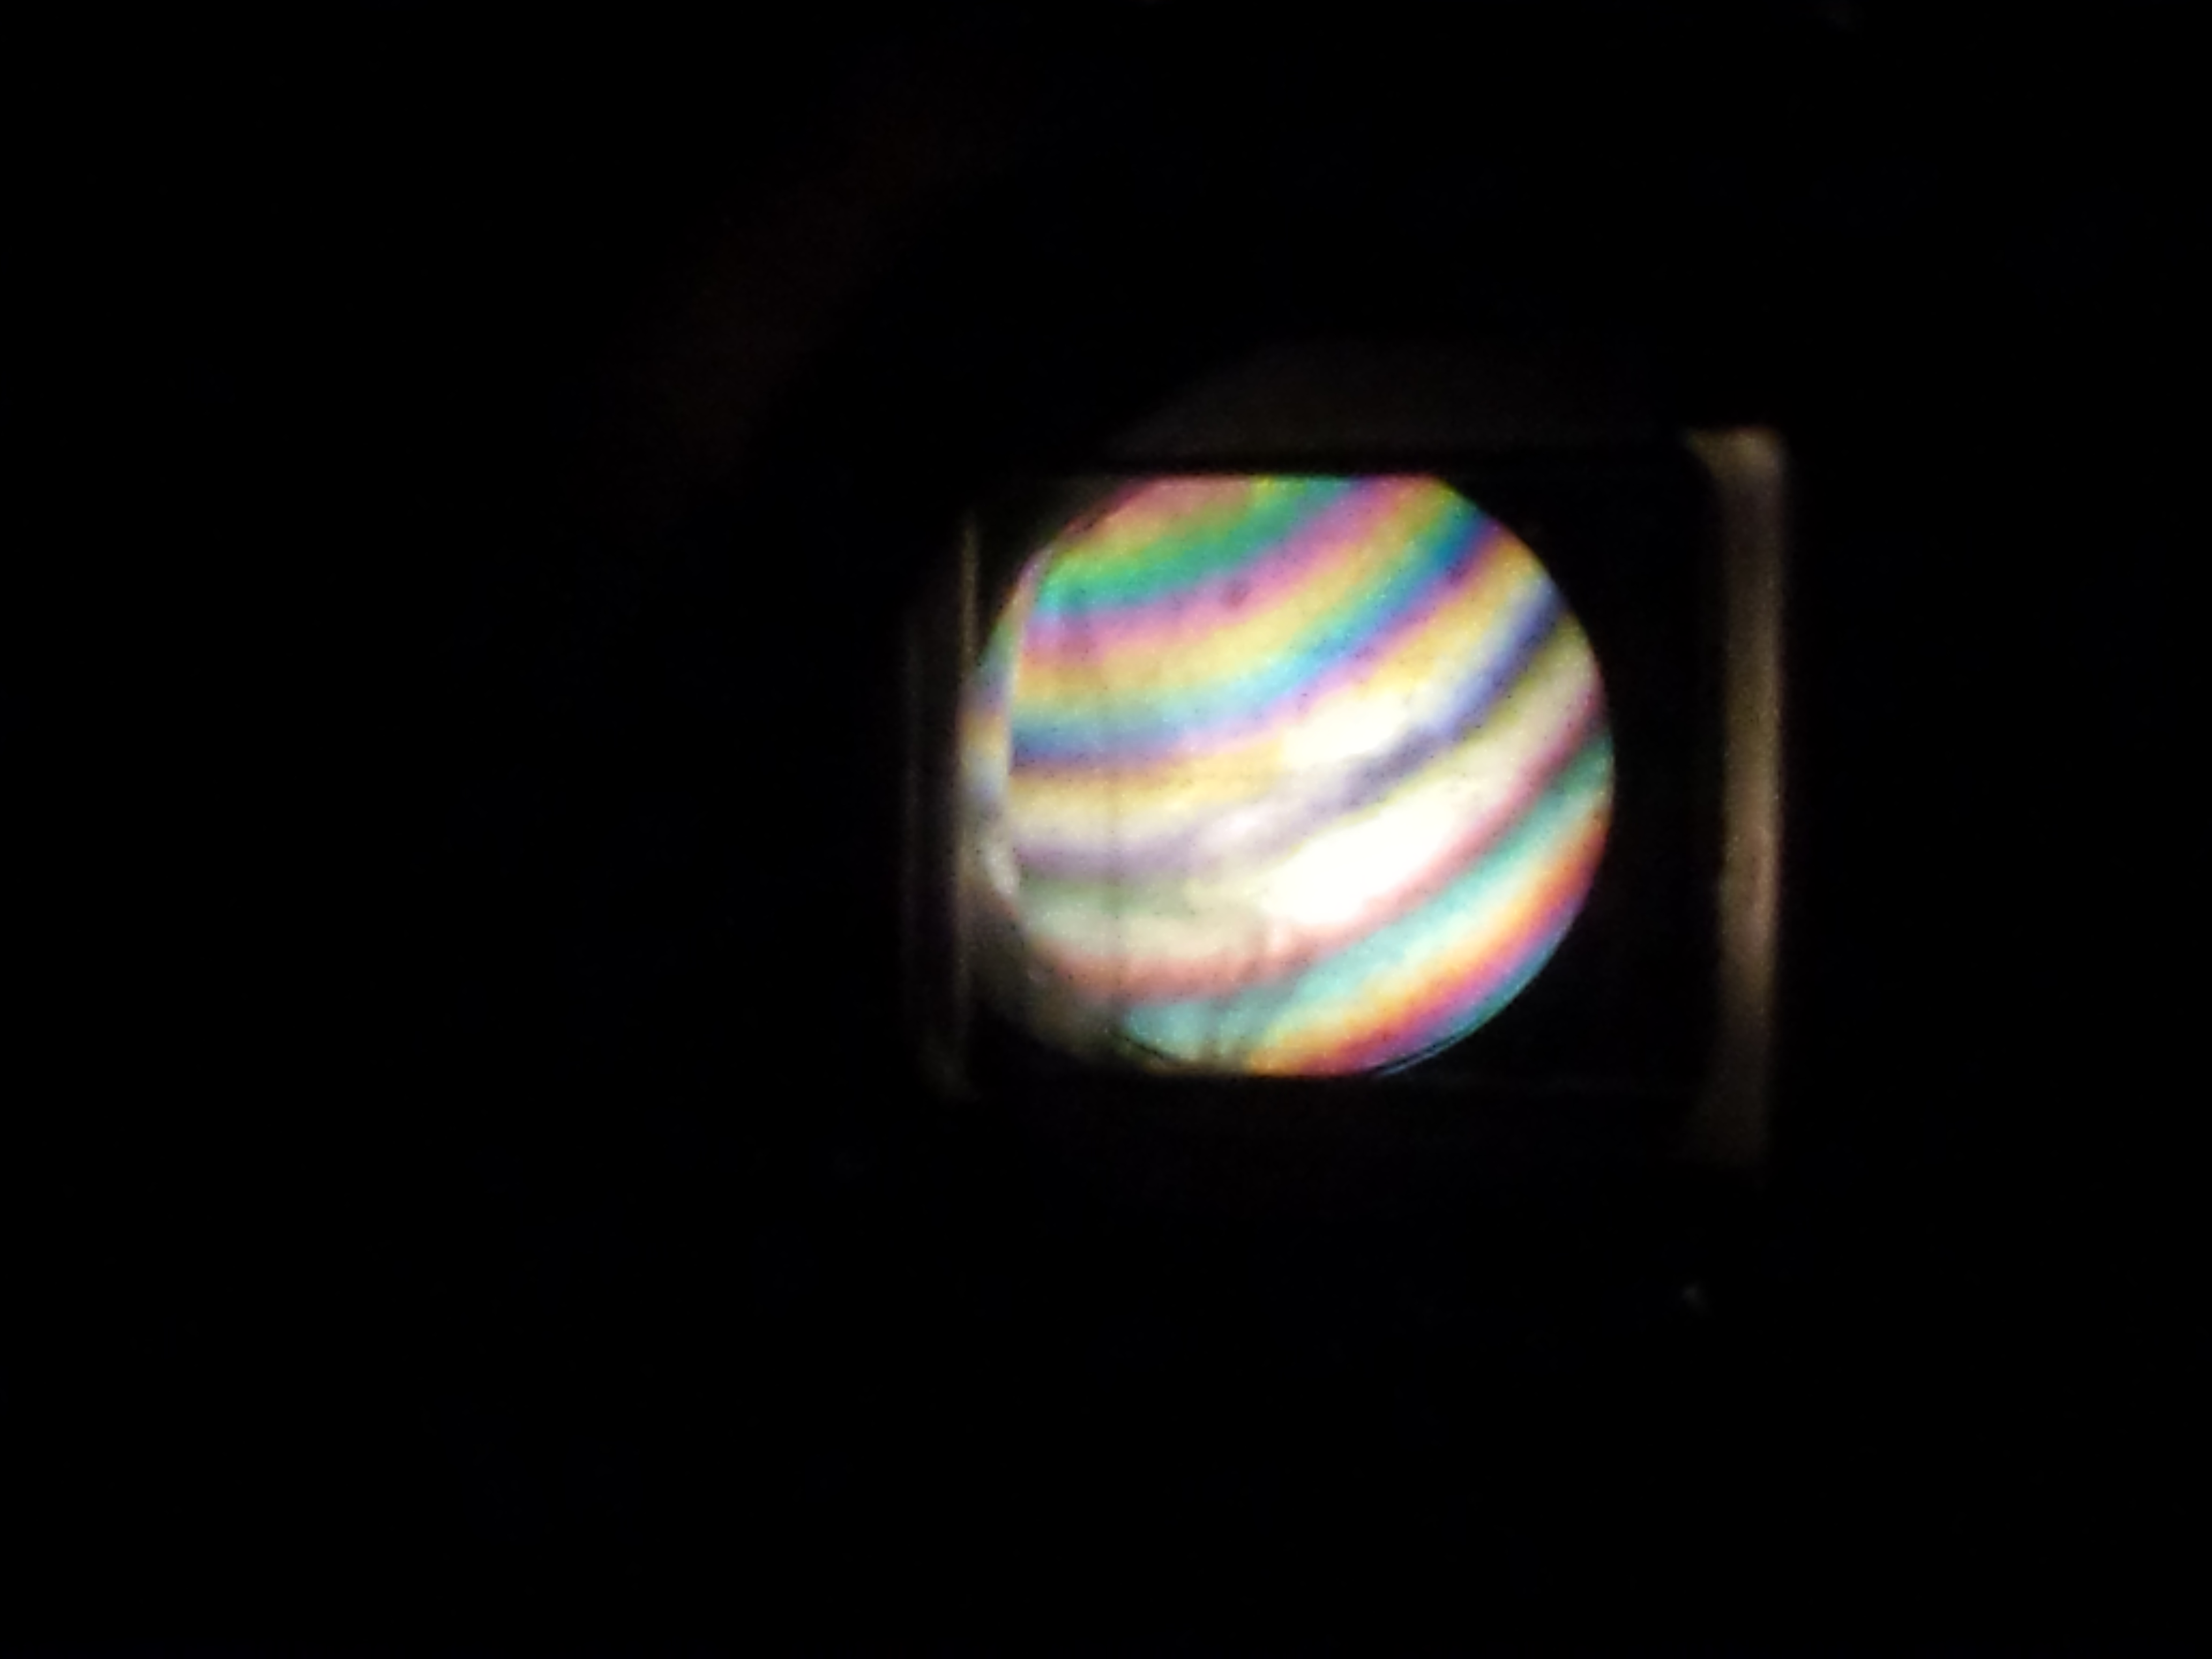
\includegraphics[scale=0.5]{frange_bianca.pdf}
	\caption{Frange determinate dalla luce bianca osservate all'uscita dell'interferometro}
           \label{f:frange_bianca}
\end{figure}